\subsection{Vergleich von \bothAlgs}
\label{chap:vergleich}

Die Algorithmen \bothAlgs haben zwei zentrale Unterschiede. 
Zum einen die Aktion des Folgezustands und somit der Q-Value, der für das Update genutzt wird. 
Zum anderen der Zeitpunkt, zu dem das Update durchgeführt wird \cite{IrelandComparisonThereFundamental}. 
Sarsa nutzt für das Update die Aktion, die es gemäß seiner Policy auswählt. 
Hingegen nutzt Q-Learning für das Update immer die Aktion mit dem höchsten Q-Value, auch wenn es gemäß Policy eine andere Aktion ausführt. 
Aufgrund dessen wird Sarsa als ein On-Policy und Q-Learning als ein Off-Policy Algorithmus klassifiziert \cite[S. 132]{suttonReinforcementLearningIntroduction2018}.

Zur Veranschaulichung des Unterschiedes wird das Update von Sarsa und Q-Learning am Beispiel von Gridworld erklärt. 
\cref{fig:gridworld_sample} zeigt die $\epsilon$-greedy-Policy, nach der beide Agent mit der Umgebung interagieren. 
Die State-Transition Probability und Rewardfunktion sind unverändert, aber den Agenten nicht bekannt.
Es gilt $\gamma=0,9$ und $\alpha=0,1$.
Der blaue Pfeil zeigt den Pfad einer Episode für beide Agenten. 
\cref{tab:tdlexample} enthält einen Ausschnitt einer willkürlich gefüllten Q-Tabelle für die Zustände C1 und C2.

\begin{minipage}{\textwidth}
  \begin{minipage}[b]{0.49\textwidth}
    \centering
    \captionsetup{type=figure}
    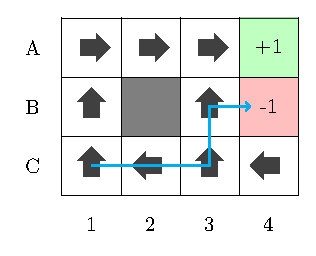
\includegraphics[]{gridworld/gridworld_sample.pdf}
    \captionof{figure}[Sample Episode für Gridworld]{Sample Episode für Gridworld\protect\footnotemark}
    \label{fig:gridworld_sample}
  \end{minipage}
  \hfill
  \begin{minipage}[b]{0.49\textwidth}
    \centering
    \captionsetup{type=table}
    % \begin{table}
\begin{tabular}{llr}
\toprule
Zustand $S$ & Aktion $A$    & $Q(S,A)$ \\ \midrule
C1          & Norden        & 10,5     \\
            & Westen        & 5,0      \\
            & Süden         & 8,7      \\
            & Osten         & 0,1      \\ \cmidrule{1-3}
C2          & Norden        & 8,2      \\ 
            & Westen        & -2,0     \\
            & Osten         & 9,8      \\
            & Süden         & 6,5      \\ \bottomrule
\end{tabular}
% \end{table}
% \begin{table}
% \centering
% \caption{\qtable mit Beispieleinträgen für Gridworld}
% \label{tab:qtable_tdl_example}

% \begin{tabular}{llr}
% \toprule
% Zustand $S$ & Aktion $A$    & $Q(S,A)$ \\ \midrule
% C1          & Norden        & 10,5     \\
%             & Westen        & 5,0      \\
%             & Süden         & 8,7      \\
%             & Osten         & 0,1      \\ \cmidrule{1-3}
% C2          & Norden        & 8,2      \\ 
%             & Westen        & -2,0     \\
%             & Osten         & 9,8      \\
%             & Süden         & 6,5      \\
% $\vdots$    & $\vdots$      & $\vdots$ \\ \bottomrule
% \end{tabular}
% \end{table}
    \captionof{table}{Willkürlich gefüllte \qtable für Gridworld}
    \label{tab:tdlexample}
    \end{minipage}
\end{minipage}
\footnotetext{eigene Darstellung in Anlehnung an \cite[S. 127]{kontesg.SeminarReinforcementLearning2021}}

Im Zustand C1 wählt der Agent die Greedy-Aktion “Norden”. Wegen der Transposition-Probability wechselt der Agent jedoch in den Zustand C2. Im Zustand C2 ist die Greedy-Aktion “Osten”. Der Agent wählt aufgrund von $\epsilon$-greedy zufällig die Aktion “Westen”. Das Sample $(S_t,A_t,R_{t+1},S_{t+1},A_{t+1})$ der Umgebung ist somit: $(C1;N;-0,1;C2;W)$ 

Der Sarsa-Agent führt das Update in \cref{eq:sarsa_update_example} durch. Hingegen wählt der Q-Learning Agent für den Folgezustand die Aktion mit höchstem Q-Value $Q(C2,Osten)=9,8$ führt daher das Update aus \cref{eq:ql_update_example} durch.

\begin{equation}
    \label{eq:sarsa_update_example}
    \equationentry{Beispiel TD Update Sarsa}
    \begin{split}
    Q(C1,N) & =Q(C1,N)+\alpha[-0,01+0,09Q(C2, W)-Q(C1,N)] \\
    Q(C1,N) & =10,5+0,1[-0,1+0.9(-2,0)-10.5]=9,26
    \end{split}
\end{equation}

\begin{equation}
    \label{eq:ql_update_example}
    \equationentry{Beispiel TD Update Q-Learning}
    \begin{split}
        Q(C1,N) &=Q(C1,N)+\alpha[-0,01+0,09Q(C2, O)-Q(C1,N)]\\
        Q(C1,N) &=10,5+0,1[-0,1+0.9(9,8)-10.5]=10,32
    \end{split}
\end{equation}



Würden beide Algorithmen einer Greedy-Policy folgen, wäre das Update gleich. 
Während Sarsa seine Aktion $A_{t+1}$ vor dem Update ausgewählt hat, wählt Q-Learning diese erst, nachdem das Update durchgeführt wurde. 
In Situationen, in denen ein Zustand der eigene Folgezustand ist, könnten Q-Learning und Sarsa unterschiedliche Aktionen $A_{t+1}$ auswählen, da sich die \qValues der Aktionen durch das Update geändert haben könnten. \cite{IrelandComparisonThereFundamental}

Ein weiteres Beispiel, dass den Unterschied von Q-Learning und Sarsa verdeutlicht ist \gqq{Cliff Walking} in \cref{fig:cliffwalking}. 
Bei diesem soll ein Agent vom Startbereich “S” zum Ziel “G” laufen. 
In jedem Zeitschritt erhalten die Agenten einen Reward $-1$, sodass sie das Ziel möglichst schnell erreichen sollen. 
Betritt ein Agent den Bereich Klippe, erhält dieser einen Reward von $-100$. 
Die Agenten können sich wieder in alle vier Himmelsrichtungen bewegen. 
Im Gegensatz zur Gridworld sind die Zustandsübergänge deterministisch. 
Die Algorithmen Q-Learning und Sarsa lernen beide mittels einer $\epsilon$-greedy-Policy mit konstantem $\epsilon$=0,1. 
Die Abbildung zeigt den optimalen Pfad (rot) und den sicheren Pfad (blau), der einen geringeren Return erzielt, aber mit größerer Wahrscheinlichkeit im Ziel ankommt. 
Während des Trainings lernt Q-Learning den optimalen Pfad, betritt jedoch aufgrund von $\epsilon=0,1$ regelmäßig die Klippe. 
Hingegen lernt Sarsa den sicheren Pfad, da es im Update die aktuelle Policy beachtet. 
Konvergiert $\epsilon$ während dem Training gegen 0 lernt Sarsa ebenfalls den optimalen Pfad. \cite[S. 132]{suttonReinforcementLearningIntroduction2018}

\begin{figure}[h]
    \centering
    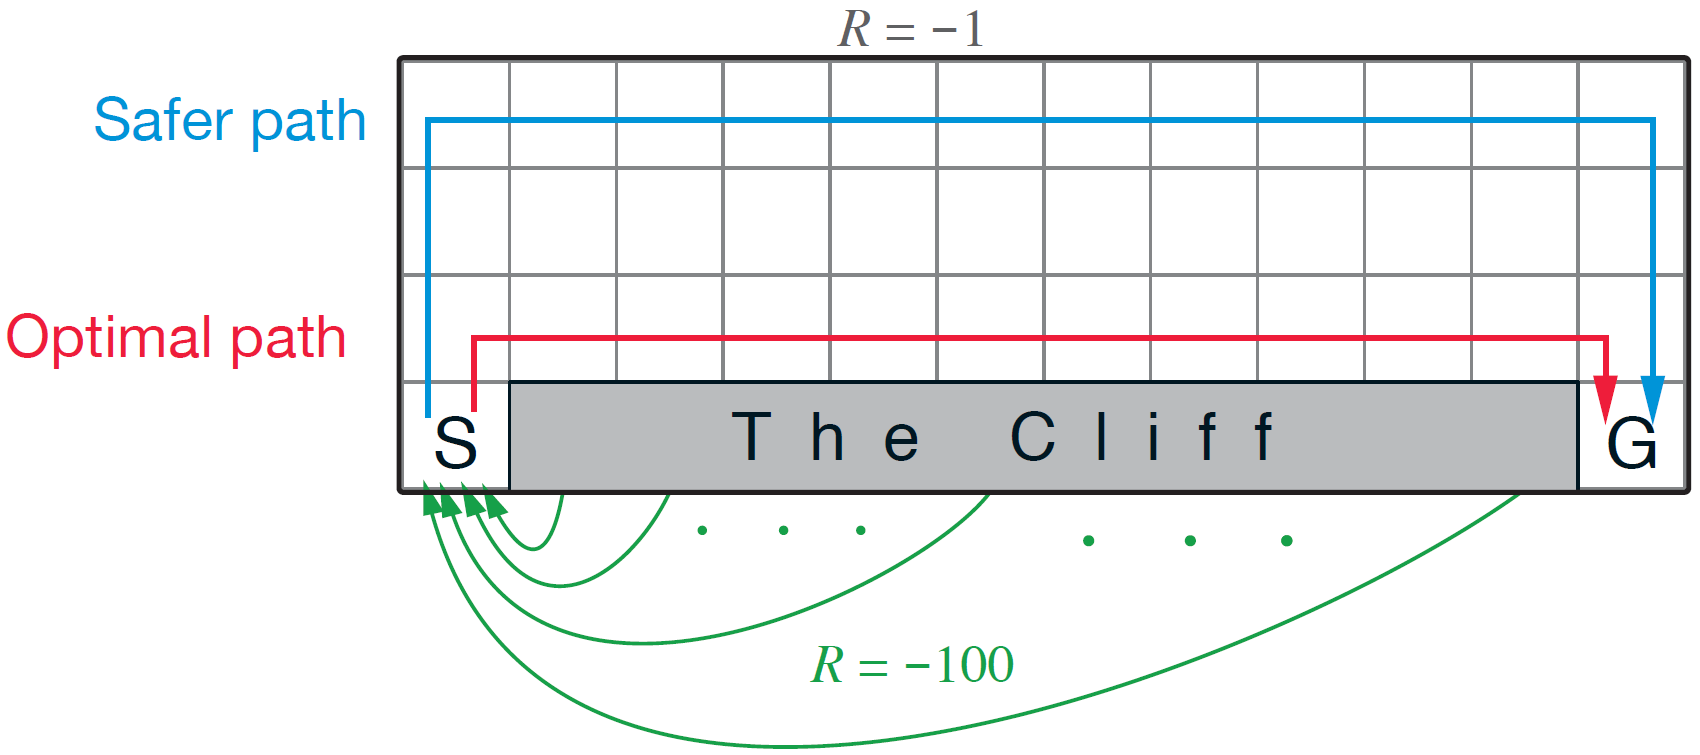
\includegraphics[scale=0.2]{04_Artefakte/01_Abbildungen/rl/rl_cliff_environment.png}
    \caption[Cliff Walking]{Cliff Walking\protect\footnotemark}
    \label{fig:cliffwalking}
\end{figure}
\footnotetext{Abbildung entnommen aus \cite[S. 132]{suttonReinforcementLearningIntroduction2018}}

Beide Algorithmen haben jedoch die gleichen Limitierungen. Da beide Algorithmen durch Interaktion mit der Umgebung lernen, werden hinreichend viele Samples benötigt, um die Action-Value Funktion zu approximieren. 
Zudem spielt die Wahl der Lernrate eine entscheidende Rolle für den Trainingserfolg. \cite[S. 131]{kontesg.SeminarReinforcementLearning2021}
Da für jedes \ac{SA Tupel} ein eigener Eintrag in der Q-Tabelle vorhanden sein muss, haben die Algorithmen zwei weitere Limitierungen.
Erstens, können beide Algorithmen nur für Probleme genutzt werden, bei denen eine Verwaltung der zu speichernden \ac{SA Tupel} praktikabel ist.
Zweitens können die Algorithmen nur optimale Entscheidungen treffen, wenn sie die \ac{SA Tupel} kennen. 
Eine Generalisierung der gesammelten Erfahrung auf neue Zustände ist nicht möglich. 
Um beide Limitierungen zu beheben können die Algorithmen mit neuronalen Netzten verknüpft werden.
Diese werden dann genutzt, um die \statevalueFunktion zu approximieren und so keine \ac{SA Tupel} speichern zu müssen und gesammelte Erfahrung zu generalisieren. \cite[S. 195f.]{suttonReinforcementLearningIntroduction2018}, \cite[S. 137ff.]{kontesg.SeminarReinforcementLearning2021}